\begin{table*}[h!]
\vspace{-0.8cm}
%  \centering
	\begin{subtable}{\textwidth}
        \centering
        {\renewcommand{\arraystretch}{0.7}
                                \begin{tabular}{ c@{\hspace{3pt}} c@{\hspace{3pt}} c@{\hspace{3pt}} c@{\hspace{3pt}} c}				
						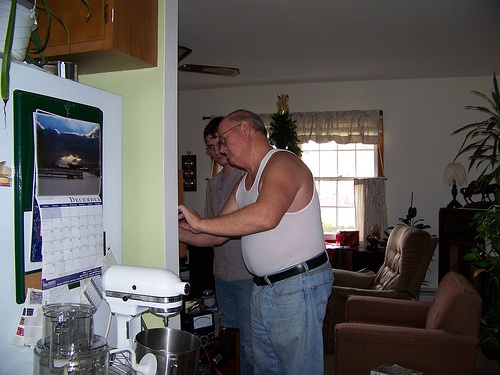
\includegraphics[width=0.19\textwidth]{figs/pascal/original/144.jpg}%
						& 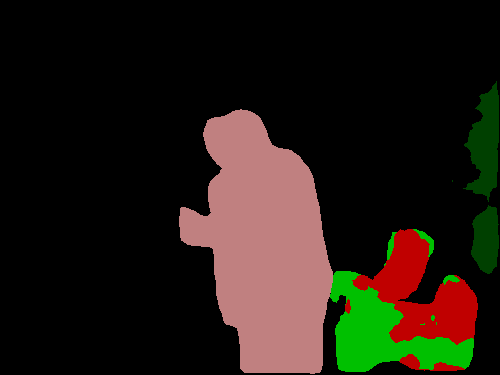
\includegraphics[width=0.19\textwidth]{figs/pascal/before_sem/144.png}%
						& 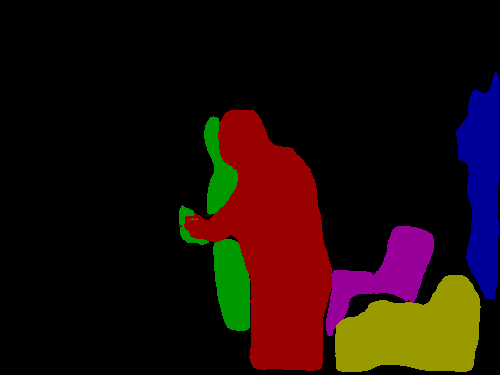
\includegraphics[width=0.19\textwidth]{figs/pascal/before_ins/144.png}%
						& 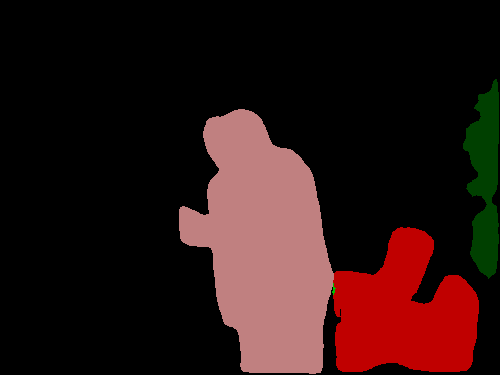
\includegraphics[width=0.19\textwidth]{figs/pascal/after_sem/144.png}%
						& 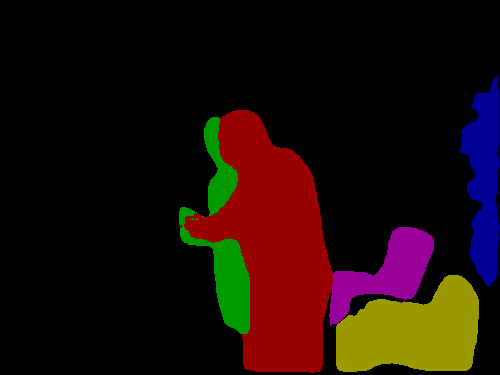
\includegraphics[width=0.19\textwidth]{figs/pascal/after_ins/144.png}\\
														\newline
						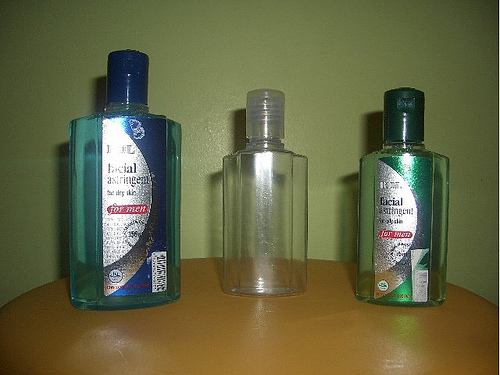
\includegraphics[width=0.19\textwidth]{figs/pascal/original/421.jpg}%
						& 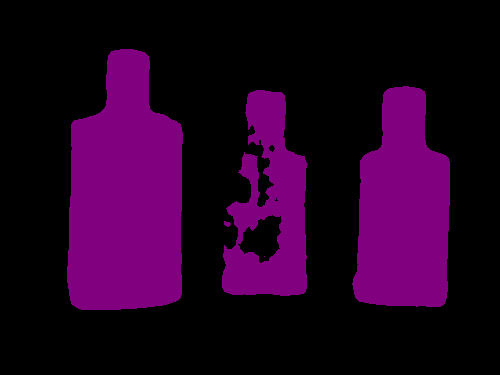
\includegraphics[width=0.19\textwidth]{figs/pascal/before_sem/421.png}%
						& 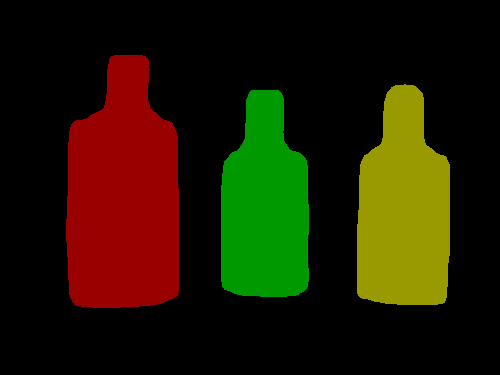
\includegraphics[width=0.19\textwidth]{figs/pascal/before_ins/421.png}%
						& 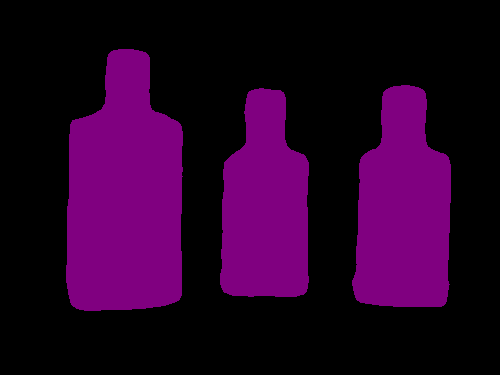
\includegraphics[width=0.19\textwidth]{figs/pascal/after_sem/421.png}%
						& 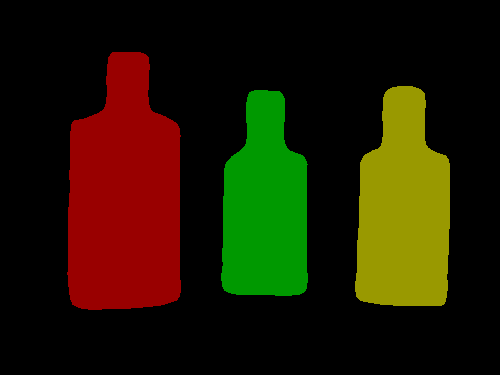
\includegraphics[width=0.19\textwidth]{figs/pascal/after_ins/421.png}\\
						                                \newline
						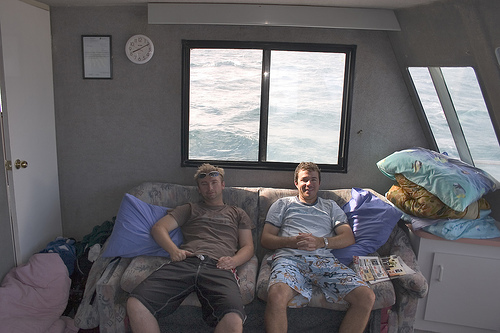
\includegraphics[width=0.19\textwidth]{figs/pascal/original/438.jpg}%
						& 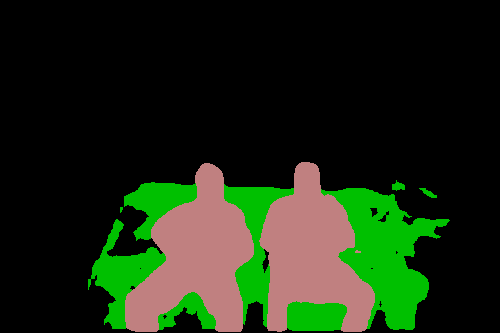
\includegraphics[width=0.19\textwidth]{figs/pascal/before_sem/438.png}%
						& 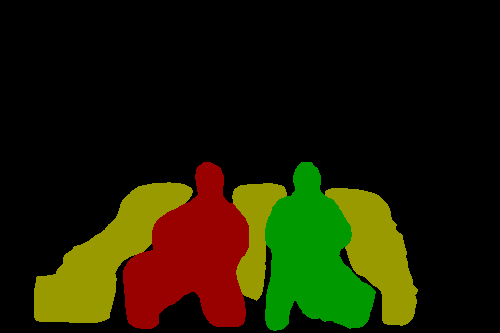
\includegraphics[width=0.19\textwidth]{figs/pascal/before_ins/438.png}%
						& 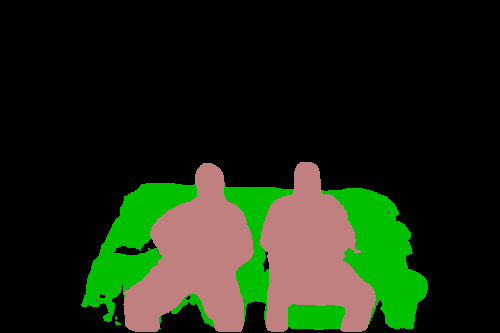
\includegraphics[width=0.19\textwidth]{figs/pascal/after_sem/438.png}%
						& 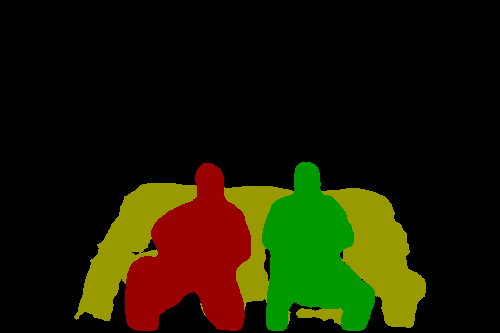
\includegraphics[width=0.19\textwidth]{figs/pascal/after_ins/438.png}\\
						                               \newline
						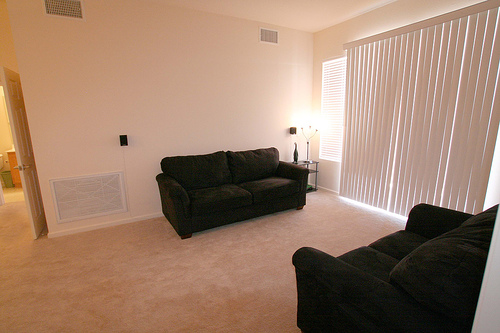
\includegraphics[width=0.19\textwidth]{figs/pascal/original/468.jpg}%
						& 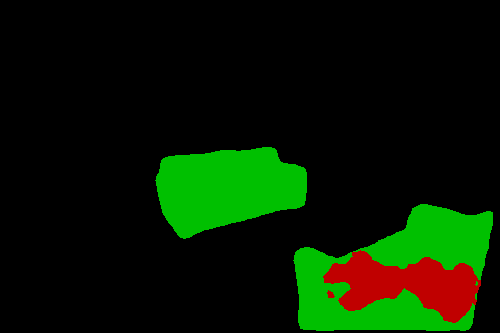
\includegraphics[width=0.19\textwidth]{figs/pascal/before_sem/468.png}%
						& 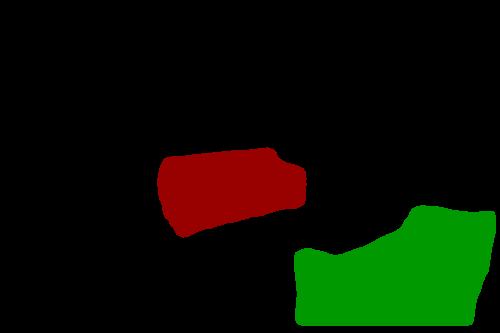
\includegraphics[width=0.19\textwidth]{figs/pascal/before_ins/468.png}%
						& 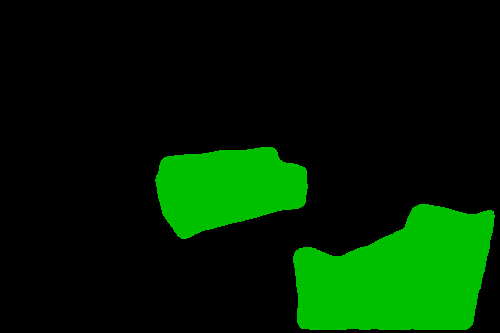
\includegraphics[width=0.19\textwidth]{figs/pascal/after_sem/468.png}%
						& 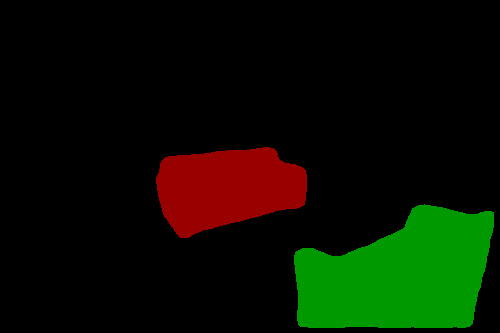
\includegraphics[width=0.19\textwidth]{figs/pascal/after_ins/468.png}\\
														\newline
						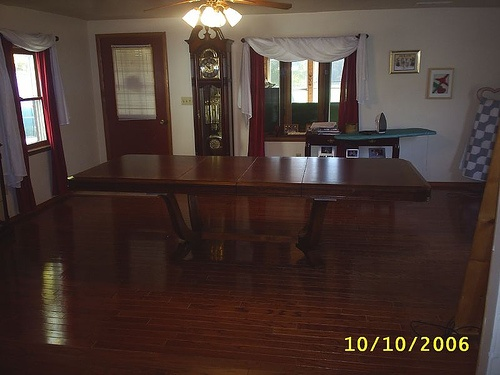
\includegraphics[width=0.19\textwidth]{figs/pascal/original/184.jpg}%
                        & 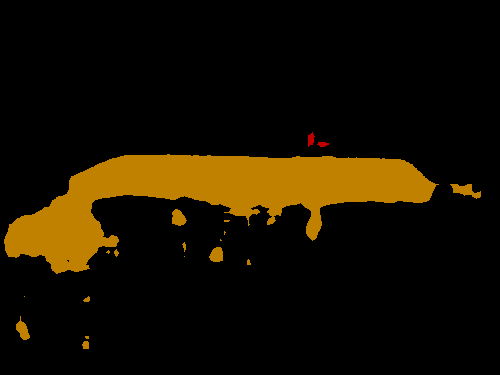
\includegraphics[width=0.19\textwidth]{figs/pascal/before_sem/184.png}%
                        & 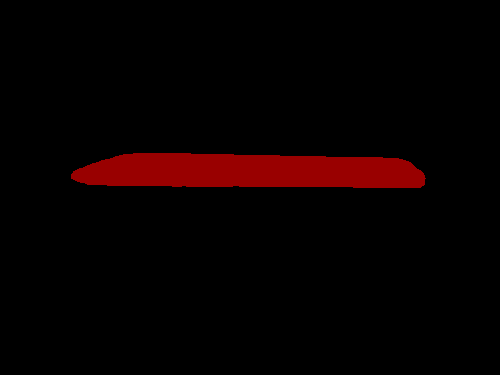
\includegraphics[width=0.19\textwidth]{figs/pascal/before_ins/184.png}%
                        & 
\includegraphics[width=0.19\textwidth]{figs/pascal/after_sem/184.png}%
                        & 
\includegraphics[width=0.19\textwidth]{figs/pascal/after_ins/184.png}\\
                                                        \newline
						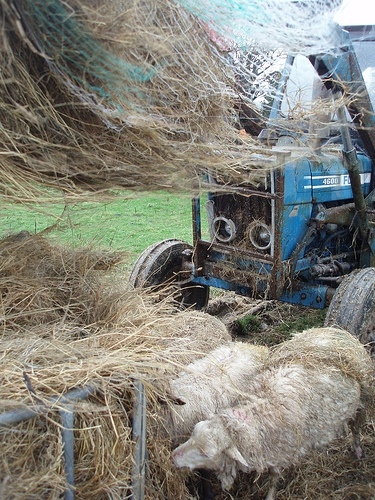
\includegraphics[width=0.19\textwidth]{figs/pascal/original/226.jpg}%
                        & 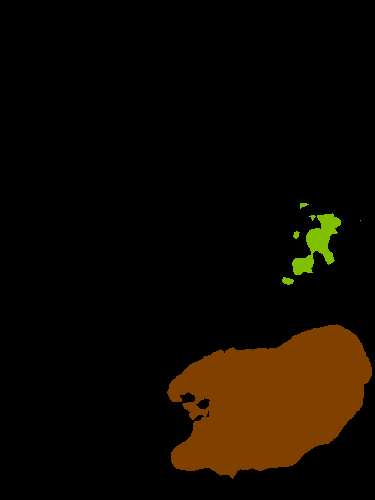
\includegraphics[width=0.19\textwidth]{figs/pascal/before_sem/226.png}%
                        & 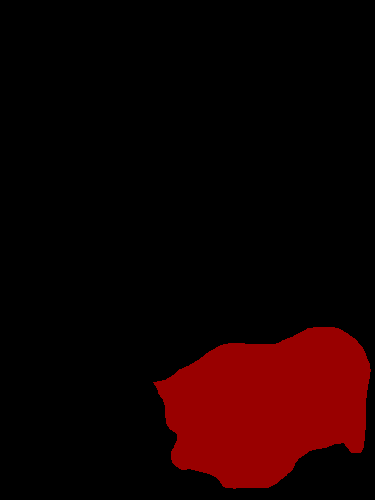
\includegraphics[width=0.19\textwidth]{figs/pascal/before_ins/226.png}%
                        & 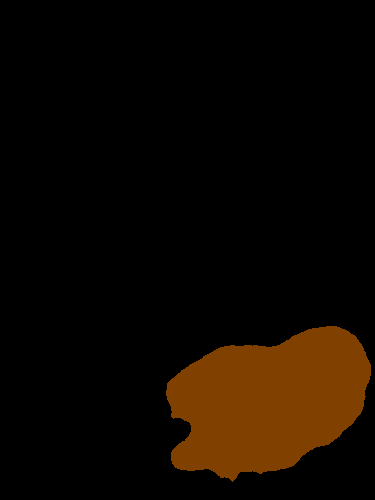
\includegraphics[width=0.19\textwidth]{figs/pascal/after_sem/226.png}%
                        & 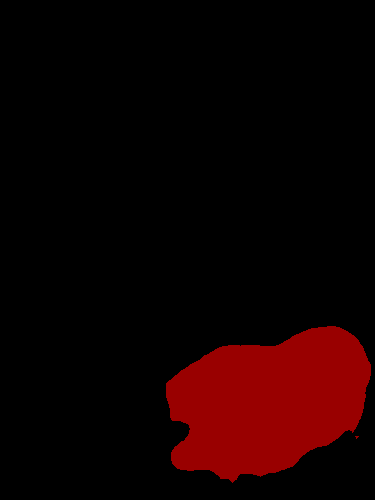
\includegraphics[width=0.19\textwidth]{figs/pascal/after_ins/226.png}\\
%                                                          \newline
%  						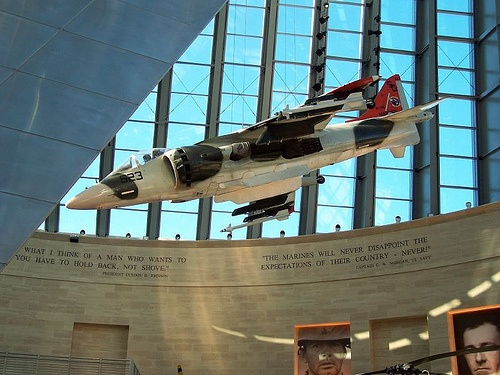
\includegraphics[width=0.19\textwidth]{figs/pascal/original/233.jpg}%
%                          & 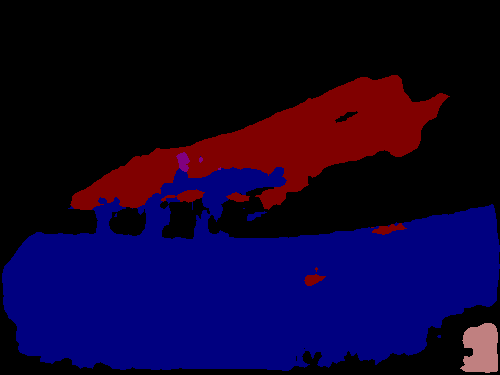
\includegraphics[width=0.19\textwidth]{figs/pascal/before_sem/233.png}%
%                          & 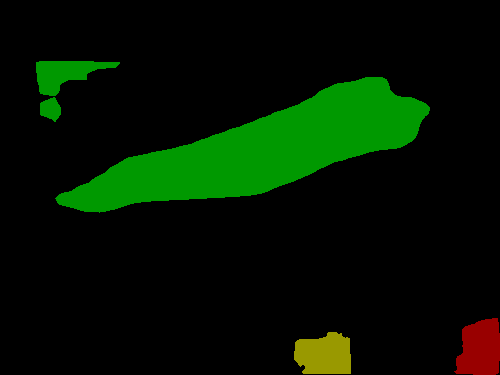
\includegraphics[width=0.19\textwidth]{figs/pascal/before_ins/233.png}%
%                          & 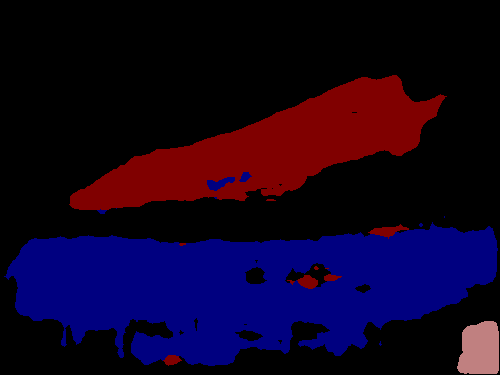
\includegraphics[width=0.19\textwidth]{figs/pascal/after_sem/233.png}%
%                          &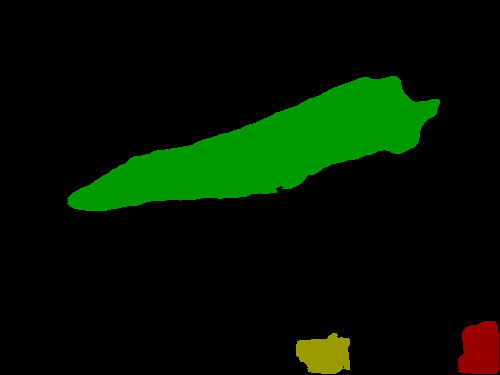
\includegraphics[width=0.19\textwidth]{figs/pascal/after_ins/233.png}\\														
% 														
                                \end{tabular}
                                }
    \end{subtable}
    \vspace{0.0cm}
    \caption[Visualizations on Pascal VOC]{{\bf Visualizations on Pascal VOC.} Example images from the Pascal VOC validation set. Columns left to right: original image, semantic output before BCRF, instance output before BCRF, semantic output after BCRF, instance output after BCRF. Each row contains a new image. The standard Pascal VOC color map is used for the semantic segmentation results.}
    \label{tbl:pascal_visual}
    \vspace{0.1cm}
\end{table*}
